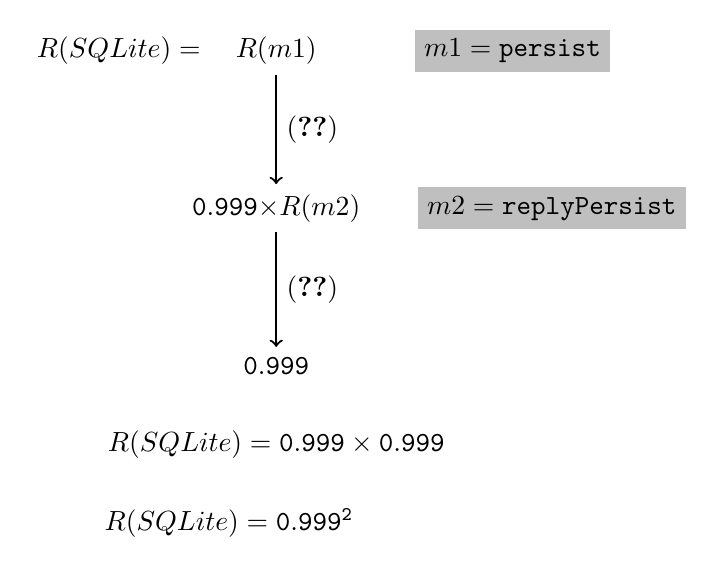
\begin{tikzpicture}[thick]
%\draw[help lines, step=1cm] (0,0) grid +(10,15);
%%%%%%%%%%%%%%%%%%%%%%%%%%%%%%% Derivation tree for SQLite
\node[rectangle, draw=none](rSqlite) at (0,15){$R(SQLite)=$};
\node[rectangle, draw=none](rM1) at (2,15){$R(m1)$};
\node[rectangle, draw=none, fill=gray!50](obsM1) at(5,15){$m1 = \mathtt{persist}$};
\node[rectangle, draw=none](rM2) at(2,13){$\mathtt{0.999 \times} R(m2)$};
\node[rectangle, draw=none, fill=gray!50](obsM1) at(5.5,13){$m2 = \mathtt{replyPersist}$};
\draw[->, thick] (rM1) -- node[draw=none, auto]{(\ref{eq:syncMessageReliability})}(rM2);
\node[rectangle, draw=none](rTerm) at(2,11){$\mathtt{0.999}$};
\draw[->, thick] (rM2) -- node[draw=none, auto]{(\ref{eq:syncMessageReliability})}(rTerm);
\node[rectangle, draw=none](rSqlite) at (2,10){$R(SQLite)= \mathtt{0.999 \times 0.999}$};
\node[rectangle, draw=none](rSqlite) at (1.4,9){$R(SQLite)= \mathtt{0.999^2}$};
\end{tikzpicture}
